
%\documentclass[12pt,english]{article}
%
%\usepackage[round]{natbib}
%% seperators
%\setcitestyle{aysep={,},yysep={,},citesep={;},notesep={: }}
%% hide boxes around hyperlinks
%\usepackage[hidelinks]{hyperref}
%\urlstyle{same}
%% customized captions for tables and figures
%\renewcommand{\thetable}{\Roman{table}}
%\usepackage{caption}\captionsetup{labelsep = period}
%
%\usepackage{setspace}
%\usepackage{vmargin}
%\usepackage{amsmath}
%\usepackage{lscape}
%\usepackage{graphicx}
%\usepackage{rotating}
%\usepackage{lscape}
%\usepackage{titling}
%\usepackage{subcaption}
%
%\usepackage{color}
%\usepackage{float}
%\usepackage{multirow}
%\usepackage{booktabs, caption, makecell}
%\usepackage{longtable}
%
%\usepackage{threeparttable}
%\usepackage{dcolumn}
%\usepackage{hanging}
%\usepackage{pdflscape}
%\pdfminorversion=4   
%
%% NOTE: To produce blinded version, replace "0" with "1" below.
%\newcommand{\blind}{1}
%
%
%\setmarginsrb{.9in}{.9in}{.9in}{.9in}{0pt}{0.25in}{0pt}{0.2in}




\chapter{Introducing the Anatomy of Resistance Campaigns (ARC) Dataset}



%\author{Charles Butcher,$^1$ $^,$ $^4$ Jessica Maves Braithwaite,$^2$ Jonathan Pinckney,$^3$ \\
% Eirin Haugseth$^1$ $^,$ $^4$,  Ingrid Vik Bakken$^1$ and Marius Swane Wishman$^1$}



\begin{abstract}

We introduce the Anatomy of Resistance Campaigns (ARC) dataset, which records
information on 1,426 organizations that participated in events of maximalist
violent and nonviolent contention in Africa from 1990-2015. The ARC data
disaggregate episodes of contention into their organizational components and
inter-organizational networks, containing 18 variables covering
organization-level features such as type, age, leadership, goals, origins,
social bases, and inter-organizational alliances. These data facilitate new
measurements of key concepts in the study of contentious politics, such as the
social and ideological diversity of resistance episodes, in addition to measures
of network centralization and fragmentation. This paper outlines the core
concepts underpinning the ARC data, the data collection method, and descriptive
statistics that illustrate trends in organizational participation over time and
how organization types vary in their main features. The paper also provides
initial evidence that structural factors correlate with the participation of
some organization types, but not others. Finally, we show how organization types
cluster together or repel each other during periods of contention. The ARC
dataset can resolve existing debates in the field and opens new avenues of
inquiry in the study of contentious dissent. It should be useful to scholars of
violent and nonviolent contention, repression and dissent, along with
researchers aiming to understand the dynamics of revolution and democratization. 

\end{abstract}

\textbf{Keywords:} organizations, networks, protest, dissent, civil war, data \\

\pagebreak

Most resistance movements are comprised of organizations that mobilize people,
make tactical decisions, issue demands, and accept or reject concessions
\citep{Haggard2016, Metternich2013, Braithwaite2020, Cunningham2017a,
McAdam2010, Tarrow2011}. Organizations often head transitional regimes, assume
power after post-conflict elections, and re-mobilize when democratic
institutions are threatened \citep{Haggard2016, Wood2000}. However, we lack
systematic cross-national data on dissident organizations spanning a variety of
tactics, goals, and group identities. 

This matters because organizational dynamics are often central to theories of
the onset, dynamics, and outcomes of violent and nonviolent resistance campaigns
\citep{Bethke2019a, Brancati2016, Chenoweth2011, Celestino2013, Huang2016,
Schaftenaar2017, Thurber2019, Sutton2014, Svensson2011, Belgioioso2018}.
Empirical analyses, however, usually depend on broad indicators of contention
summarized over a campaign or campaign-year \citep{Chenoweth2011}, which leaves
uncertainty around whether the theorized mechanisms drive observed effects
\citep{Schock2005}. Case studies show that resistance campaigns involve complex
networks of organizations and social groups \citep{Metternich2013, Schock2005,
Osa2003} and demonstrate -- with detailed assessments of actors and their
characteristics -- that the features of these organizations and networks help
explain tactical choices, campaign outcomes, and democratization
\citep{Pearlman2011, Thurber2019, Nepstad2011, Schock2005, Wood2000,
Collier1999}. Yet, it is difficult to generalize these findings to a larger
sample of cases.  

The Anatomy of Resistance Campaigns (ARC) dataset provides information on 1,426
distinct organizations across 3,407 organization-country-years associated with
events of `maximalist' collective dissent in Africa from 1990-2015. ARC includes
information on organization types, origins, leadership, mobilization bases,
goals, network ties, relationships with the state, and more. These data enable
detailed observations of actor- and network-level characteristics across a large
sample of cases, allowing scholars to unpack the organizational composition of
resistance campaigns and their network structures. The ARC data can help answer
lingering questions: how do ideological diversity and unity (through fronts and
alliances) impact campaign outcomes and post-conflict institutional change
\citep{Chenoweth2011, Bayer2016, Celestino2013}? Are some campaigns more
resilient to repression than others because of their network structures or the
nature of participating organizations \citep{Sutton2014, Siegel2009}? How do
coalitions evolve through periods of institutional reform -- especially
democratic transitions \citep{Pinckney2020}? To the extent that data
availability shapes theoretical horizons \citep{Gleditsch2014}, ARC can
stimulate additional research questions in myriad areas.

\section{Core concepts in ARC}

The ARC dataset focuses on \emph{organizations} that participated in acts of
\emph{collective dissent} for goals of \emph{maximalist} change.
\textit{Organizations} are structures designed to cohere people and resources -
often through collective action - to pursue common goals \citep[2]{North1990,
Daft1992}. The presence of a formal structure (however thin the hierarchy)
intended to aggregate individual efforts towards a defined goal distinguishes
organizations from broad social categories such as ``students,'' ``protesters,''
or the ``working class.'' We discuss our operationalization of this concept in a
subsequent section.    

\emph{Collective dissent} is observable action involving multiple people, beyond
normal institutional procedures for realizing political goals \citep{Tilly1978}.
This ranges from demonstrations and strikes to rebellion and terrorist attacks,
while excluding actions lacking a clear political goal and everyday or
institutional political activities such as lobbying politicians or electoral
participation. Organizations engage in collective dissent when they deploy their
mobilization infrastructure to encourage individual participation in these
events.  

We define \emph{maximalist} demands as calls for changes in the political
structure that would significantly alter the executive's access to state power,
the rules with which executives are selected, or the policy or geographic areas
for which the executive has the right to make laws. Examples of maximalism
include demands that a head of state resign via a non-institutional method, for
democratization in autocratic settings, to enfranchise an excluded social group,
and for regional or ethnic autonomy or independence.\footnote{A series of
borderline demands and their treatment can be found at the ARC project website.}

Maximalist demands exclude calls that fall short of altering these fundamental
aspects of executive power, such as improved human rights protections or changes
in public spending. Demands by a disenfranchised group for better protections
can be addressed with legislation that typically does not change the process for
deciding who holds executive power or who has lawmaking authority. Demands for
enfranchisement of that excluded group are maximalist because -- if implemented
-- they would include a new group in the process of deciding who holds executive
power. 


\section{Relationship to existing datasets}

ARC is distinct from existing resources because it provides information on the
features of organizations that participated in nonviolent \textit{and} violent
dissent, while also going beyond self-determination or ethnonationalist
movements \citep{Wilkenfeld2011, Cunningham2020}, or armed rebel groups
\citep{Pettersson2020a, Harbom2008, Braithwaite2020, Stewart2018,
Cunningham2013, Svensson2018, Cunningham2009a}. Events datasets often identify
participating actors, but lack information on their features
\citep{Chenoweth2018, Chenoweth2019b, Salehyan2012, Clark2021, Raleigh2010,
Chenoweth2019b}. The Revolutionary and Militant Organizations Dataset does
provide information about resistance organizations but seems to oversample on
violent organizations (75\% of REVMOD organization-years are rebel or terrorist
groups) and does not account for relationships between organizations
\citep{Acosta2019}. ARC is unique in capturing inter-organizational ties that
help us understand network structures in resistance episodes. 


\section{Creating ARC}

To construct the ARC dataset, we first identified organizations that
participated in events of maximalist collective dissent and then recorded
information on the features of those organizations. To maximize transparency and
replicability, coding decisions at each step were recorded in RMarkdown
files.\footnote{Markdown files available on request.}

\subsection{Identifying participants}

Participating organizations were identified by drawing on five events datasets:
the UCDP Georeferenced Event Dataset \citep{Sundberg2013}, the Social Conflict
Analysis Dataset \citep{Salehyan2012}, the Mass Mobilization Dataset
\citep{Clark2021}, the Armed Conflict Location Event Dataset
\citep{Raleigh2010}, and the NAVCO 3.0 data covering African countries
\citep{Chenoweth2018}. Together, these datasets provide a comprehensive
catalogue of nonviolent and violent collective dissent across Africa. We began
by creating a list of \emph{candidate} maximalist events by sub-setting on
variables related to dissident demands and a customized text-matching string. 

We then determined whether event participants made maximalist demands and
whether one or more named organizations participated by conducting newswire
searches in FACTIVA and LexisNexis using a targeted search string. Event IDs
from the events datasets are stored with the organization-year observations in
ARC, allowing users to integrate variables from events data with ARC. 

We added the constituent organizations of ``fronts'' according to a ``three
year'' rule. Fronts are distinct, umbrella organizations coordinating the
actions of member organizations. Some projects like the UCDP treat fronts as
unitary actors, but this obscures variation in the preferences and features of
member organizations. However, always treating fronts as decentralized
organizational networks can be impractical - and empirically inaccurate. Fronts
often become more unified over time (or they split apart) but systematically
determining when a front ceases to consist of semi-autonomous groups and becomes
a single organization is extremely difficult. We adopted an arbitrary but
empirically informed rule to resolve this issue, whereby member organizations of
a front were added as participants when those organizations had been members of
the front for three or fewer years. Member organizations were identified in
newswire databases, primary and secondary sources, and through an iterative
process when information on their features was collected by coders.  A more
detailed description of the rules for coding fronts can be found in the
codebook. 

This three year rule means that some organizations may be included that were
relatively new members of fronts but did not participate in protests, or played
only a peripheral role. However, we argue that this risk is outweighed by the
inclusion of organizations that often participate in protests but are overlooked
by news media, such as local human rights organizations, women's organizations
and youth groups. Since front participants are identified through newswires
\textit{and} primary and secondary sources, our inclusion criteria is less
subject to media biases and provides a new, more comprehensive picture of
opposition networks.


\subsection{Coding organization features}

This process produced a list of organizations linked to events of dissent.
Organization-years of maximalist dissent were then generated from the events
data and a team of coders recorded information on the features of participating
organizations. Some variables are constant across organization-years (e.g.
``birth date''), while others are dynamic. Organization-years were only coded
when organizations were identified as participating in collective dissent with
maximalist demands in a given year. Organizations often continue to exist when
they are not participating in dissent; however, their non-participation means
these observations are omitted from ARC. Constructing a full panel for
organizations between 1990-2015 is not possible for this reason and because we
do not record if and when organizations cease to exist (versus entering into
abeyance). Table \ref{Tab: Table 1} summarizes several organization-feature
variables in ARC.\footnote{The full codesheet can be found in the supplementary
materials.} 

\begin{table}[!htbp] \centering 
  \caption{Organization-level variables} 
  \label{Tab: Table 1} 
\begin{tabular}{p{3cm} p{7cm} p{6cm}} 
\\[-1.8ex]\hline 
\hline \\[-1.8ex] 
Variable & \multicolumn{1}{c}{Description} & \multicolumn{1}{c}{Format} \\
\hline \\[-1.8ex] 
\emph{Type}                     &     Categorization of organization type                                   & Categorical  \\ 
\hline \\[-1.8ex] 
\emph{Birthdate}               &     Date organization was founded                                     & Date: dd-mm-yyyy \\ 
\hline \\[-1.8ex] 
\emph{Origins}                  &     How organization formed                                         & Categorical: (Splinter, Merger, Other) \\ 
\hline \\[-1.8ex] 
\emph{Goals}                    &     Primary organization goals                                            & Open text \\ 
\hline \\[-1.8ex] 
\emph{Size}                     &     Membership size in year                                         & Numeric \\ 
\hline \\[-1.8ex] 
\emph{Size Estimate}            &     Approximate size                                                      & Ordinal \\ 
\hline \\[-1.8ex] 
\emph{Leadership}               &     Leader name/gender                                             & Open text \\ 
\hline \\[-1.8ex] 
\emph{Leadership Tenure}        &     Date leader assumed position                                     & Date: dd-mm-yyyy \\ 
\hline \\[-1.8ex] 
\emph{Leadership Ties}          &     Did leader serve at a high level in previous governments?         & Categorical: (Yes/No) \\ 
\hline \\[-1.8ex] 
\emph{Social Base}              &     Main social group(s) in organization                 & Open text \\ 
\hline \\[-1.8ex] 
\emph{Social Media}             &     Extent of social media use                               & Categorical: (None, Some, Significant) \\ 
\hline \\[-1.8ex] 
\emph{State Rel.}               &     Relationship with state at t-1                                    & Categorical \\ 
\hline \\[-1.8ex] 
\emph{Formal Ties}              &     Ties with other active organizations                & String: Organization IDs \\ 
\hline \\[-1.8ex] 
\emph{Structure I}              &     Clear leadership/decision-making structure?                           & Categorical: (Yes/No) \\ 
\hline \\[-1.8ex] 
\emph{Structure II}              &     Characterised as `decentralised'?                               & Categorical: (Yes/No) \\ 
\hline \\[-1.8ex] 
\hline \\[-1.8ex] 
\end{tabular} 
\end{table} 

ARC includes information on two types of ties between organizations: fronts and
alliances. Front ties connect a constituent organization to a higher-level
organization (a front) when the constituent organization is formally a member of
the front, or its leaders participate in the front's leadership.\footnote{In
some cases, fronts themselves become constituent organizations in higher-level
fronts. In this case, we only include ties from constituent organizations to the
closest-level front in the hierarchy.} Organizations identified by the
aforementioned ``three year'' rule have front ties to the main front.

\emph{Alliance} ties connect two or more organizations that declared they were
coordinating resistance activities, or sources indicated that organizations
coordinated efforts, but they did not form a standalone organization (front) to
manage coordination. Fronts and their constituent organizations can have
alliance ties with non-front organizations. For example, in Malawi in 1993, the
Public Affairs Committee (PAC, a front of CSOs and religious groups) allied with
the Alliance for Democracy (a political party), which was not part of PAC. Users
can assemble alliance-pairs with these front and alliance variables to explore
factors driving inter-organizational ties. 

Figure \ref{fig:arc ties} illustrates these ties. The organization at the
bottom-center has alliance ties to two other organizations and is a member of a
front. That front is also a member of another front. 

\begin{figure}
    \centering
    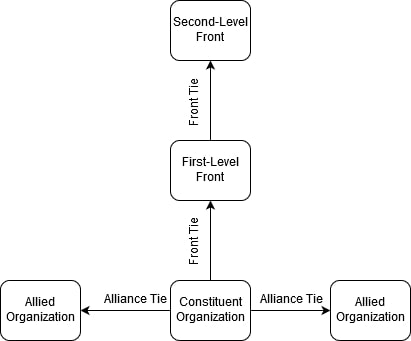
\includegraphics[width = 0.9\columnwidth]{img/example_ties.jpg}
    \caption{ARC ties example}
    \label{fig:arc ties}
\end{figure}




Our method for identifying organizations may create bias. Participation is coded
when newswires identify named organizations engaged in maximalist dissent.
Journalists may view some organizations -- especially political parties and
trade unions -- as more deserving of a proper noun. Parties are skilled at
attracting media attention and might be over-represented in reporting. Urban
organizations may also be over-represented because events in cities receive more
media coverage than events in rural locations \citep{Kalyvas2004, Eck2012,
Day2015}.\footnote{Urban organizations may also be more frequent participants
because organizations and collective action are more common in cities
\citep{Weidmann2018, Nicholls2008, Miller2013}.} Media biases could affect
inferences drawn from ARC, so robustness tests such as those from
\citet{Weidmann2016} are recommended. 

Maximalist demand-making is strategic and may occur after prior
campaign-building, after high levels of past participation in non-maximalist
protest, or when repression offers `no other way out' \citep{Goodwin2001} --
factors that independently generate regime concessions or democratization
\citep{Brancati2016, Klein2018}. Researchers should control for omitted
variables capturing these selection processes wherever possible and inferences
from ARC should be informed by the limitations of selecting on maximalist
demands.

ARC is limited to African countries from 1990-2015 for practical reasons driven
by overlap in available events datasets. However, by building on existing
datasets, we augment those resources while also maximizing compatibility.
African countries' histories of contention, civil society, and statehood are
unique and context-specific and we direct readers to studies that provide useful
background \citep{Boone2003, Branch2015, Bratton1997, Herbst2014, Mueller2018}. 

While inferences drawn from ARC only apply with confidence to the African
continent, our method of building upon existing event-based resources is
transportable to other regions, time periods, and non-maximalist dissent --
extensions we plan to offer in the future.  


Table \ref{Tab: Comparison} shows continuous measurements of ideological
diversity and opposition unity generated from ARC and compares them to similar
(but categorical) measures in the NAVCO 2.1 dataset \citep{Chenoweth2019a} from
Egypt between 2003-2015. ARC also encompasses years of democratic transition,
identifies more organizations, and enables new measurements of features such as
organization age. Figure \ref{Fig: Net1} shows a network map for Egypt in 2011,
generated using front and alliance variables in ARC.  

\clearpage

\begin{landscape}

\begin{table}[!htbp] \centering 
  \caption{Comparison of ARC and NAVCO 2.1: Egypt 2003-2015} 
  \label{Tab: Comparison} 
\begin{tabular}{cccc|cccc} 
\\[-1.8ex]\hline 
\hline \\[-1.8ex] 

 & \multicolumn{1}{c}{} & \multicolumn{1}{c}{NAVCO 2.1} &  \multicolumn{1}{c|}{} & \multicolumn{1}{c}{} & \multicolumn{1}{c}{} & \multicolumn{1}{c}{ARC}                                & \multicolumn{1}{c}{}\\
\hline \\[-1.8ex] 
Year & \multicolumn{1}{c}{Religious diversity} & \multicolumn{1}{c}{Unity$^a$} &  \multicolumn{1}{c|}{New orgs} & \multicolumn{1}{c}{No. orgs} & \multicolumn{1}{c}{Unity$^b$} & \multicolumn{1}{c}{Diversity$^g$}                                & \multicolumn{1}{c}{Mean age$^c$}\\
\hline \\[-1.8ex] 
2003 &     Yes     &                         Seemingly united   &                                      3 &                     10 &                    0.750  &         
\includegraphics[width = 0.15\columnwidth]{img/ideo2003.jpg}   &    17  \\ 

2004  &     Yes   &                             Moderate disunity   &                                   11 &                    7 &                      0.710  &        
\includegraphics[width = 0.15\columnwidth]{img/ideo2004.jpg}   &         17    \\ 

2005  &     Yes     &                        Moderate disunity   &                                      6 &                     9 &                     0.765  &        
\includegraphics[width = 0.15\columnwidth]{img/ideo2005.jpg}   &         23    \\ 

2006  &     NA   &                           NA   &                                     NA  &                   9 &                     0.793  &        
\includegraphics[width = 0.15\columnwidth]{img/ideo2006.jpg}  &          24    \\ 

2007  &     No      &                        Seemingly united   &                                      1 &                     9 &                     0.793  &        
\includegraphics[width = 0.15\columnwidth]{img/ideo2007.jpg}   &         25   \\ 

2008  &     No    &                          Moderate disunity   &                                       1 &                    2 &                     0  &            
\includegraphics[width = 0.15\columnwidth]{img/ideo2008.jpg} &           40  \\ 

2009  &     No      &                         Moderate disunity    &                                    1 &                     3 &                     1  &            
\includegraphics[width = 0.15\columnwidth]{img/ideo2009.jpg}    &        29  \\ 

2010  &     No     &                          Moderate disunity  &                                      3 &                     13 &                    0.701  &         
\includegraphics[width = 0.15\columnwidth]{img/ideo2010.jpg}  &         21   \\ 

2011  &     Yes     &                         Seemingly united  &                                      3 &                     41 &                    0.850    &          
\includegraphics[width = 0.15\columnwidth]{img/ideo2011.jpg} &       9   \\ 

2012  &     NA     &                           NA   &                                   NA &                    64 &                    0.843    &          
\includegraphics[width = 0.15\columnwidth]{img/ideo2012.jpg}  &      11   \\ 
 
2013$^d$   &     No$^f$    &                 Seemingly united$^e$   &                                    6 &                     74 &                    0.874    &          
\includegraphics[width = 0.15\columnwidth]{img/ideo2013.jpg} &       9   \\ 
 
2014  &     NA     &                           NA   &                                   NA &                    30 &                    0.901    &          
\includegraphics[width = 0.15\columnwidth]{img/ideo2014.jpg} &       9  \\ 
 
2015  &     NA      &                         NA   &                                    NA &                    15 &                     0.846    &         
\includegraphics[width = 0.15\columnwidth]{img/ideo2015.jpg} &       12   \\ 

\hline \\[-1.8ex] 
\hline \\[-1.8ex] 
\end{tabular} 
\end{table} 
\footnotesize{$^a$ Measured with the `camp\_conf\_intensity' variable. $^b$
Measured as the network centralization score, which captures the extent to which
a network coheres around (or is united by) one focal point (often a single front
in our case). $^c$ In years for valid observations. $^d$ NAVCO 2.1 features
three campaigns in 2013. $^e$ All three campaigns were `Seemingly United.'  $^f$
No religious diversity was recorded across all three campaigns. $^g$ Legend is
visualised in the network map below. Organizations that don't fit into these
categories are grey. Embedded numbers are fractionalization index scores}

\end{landscape}

\pagebreak

\begin{figure}
    \centering
    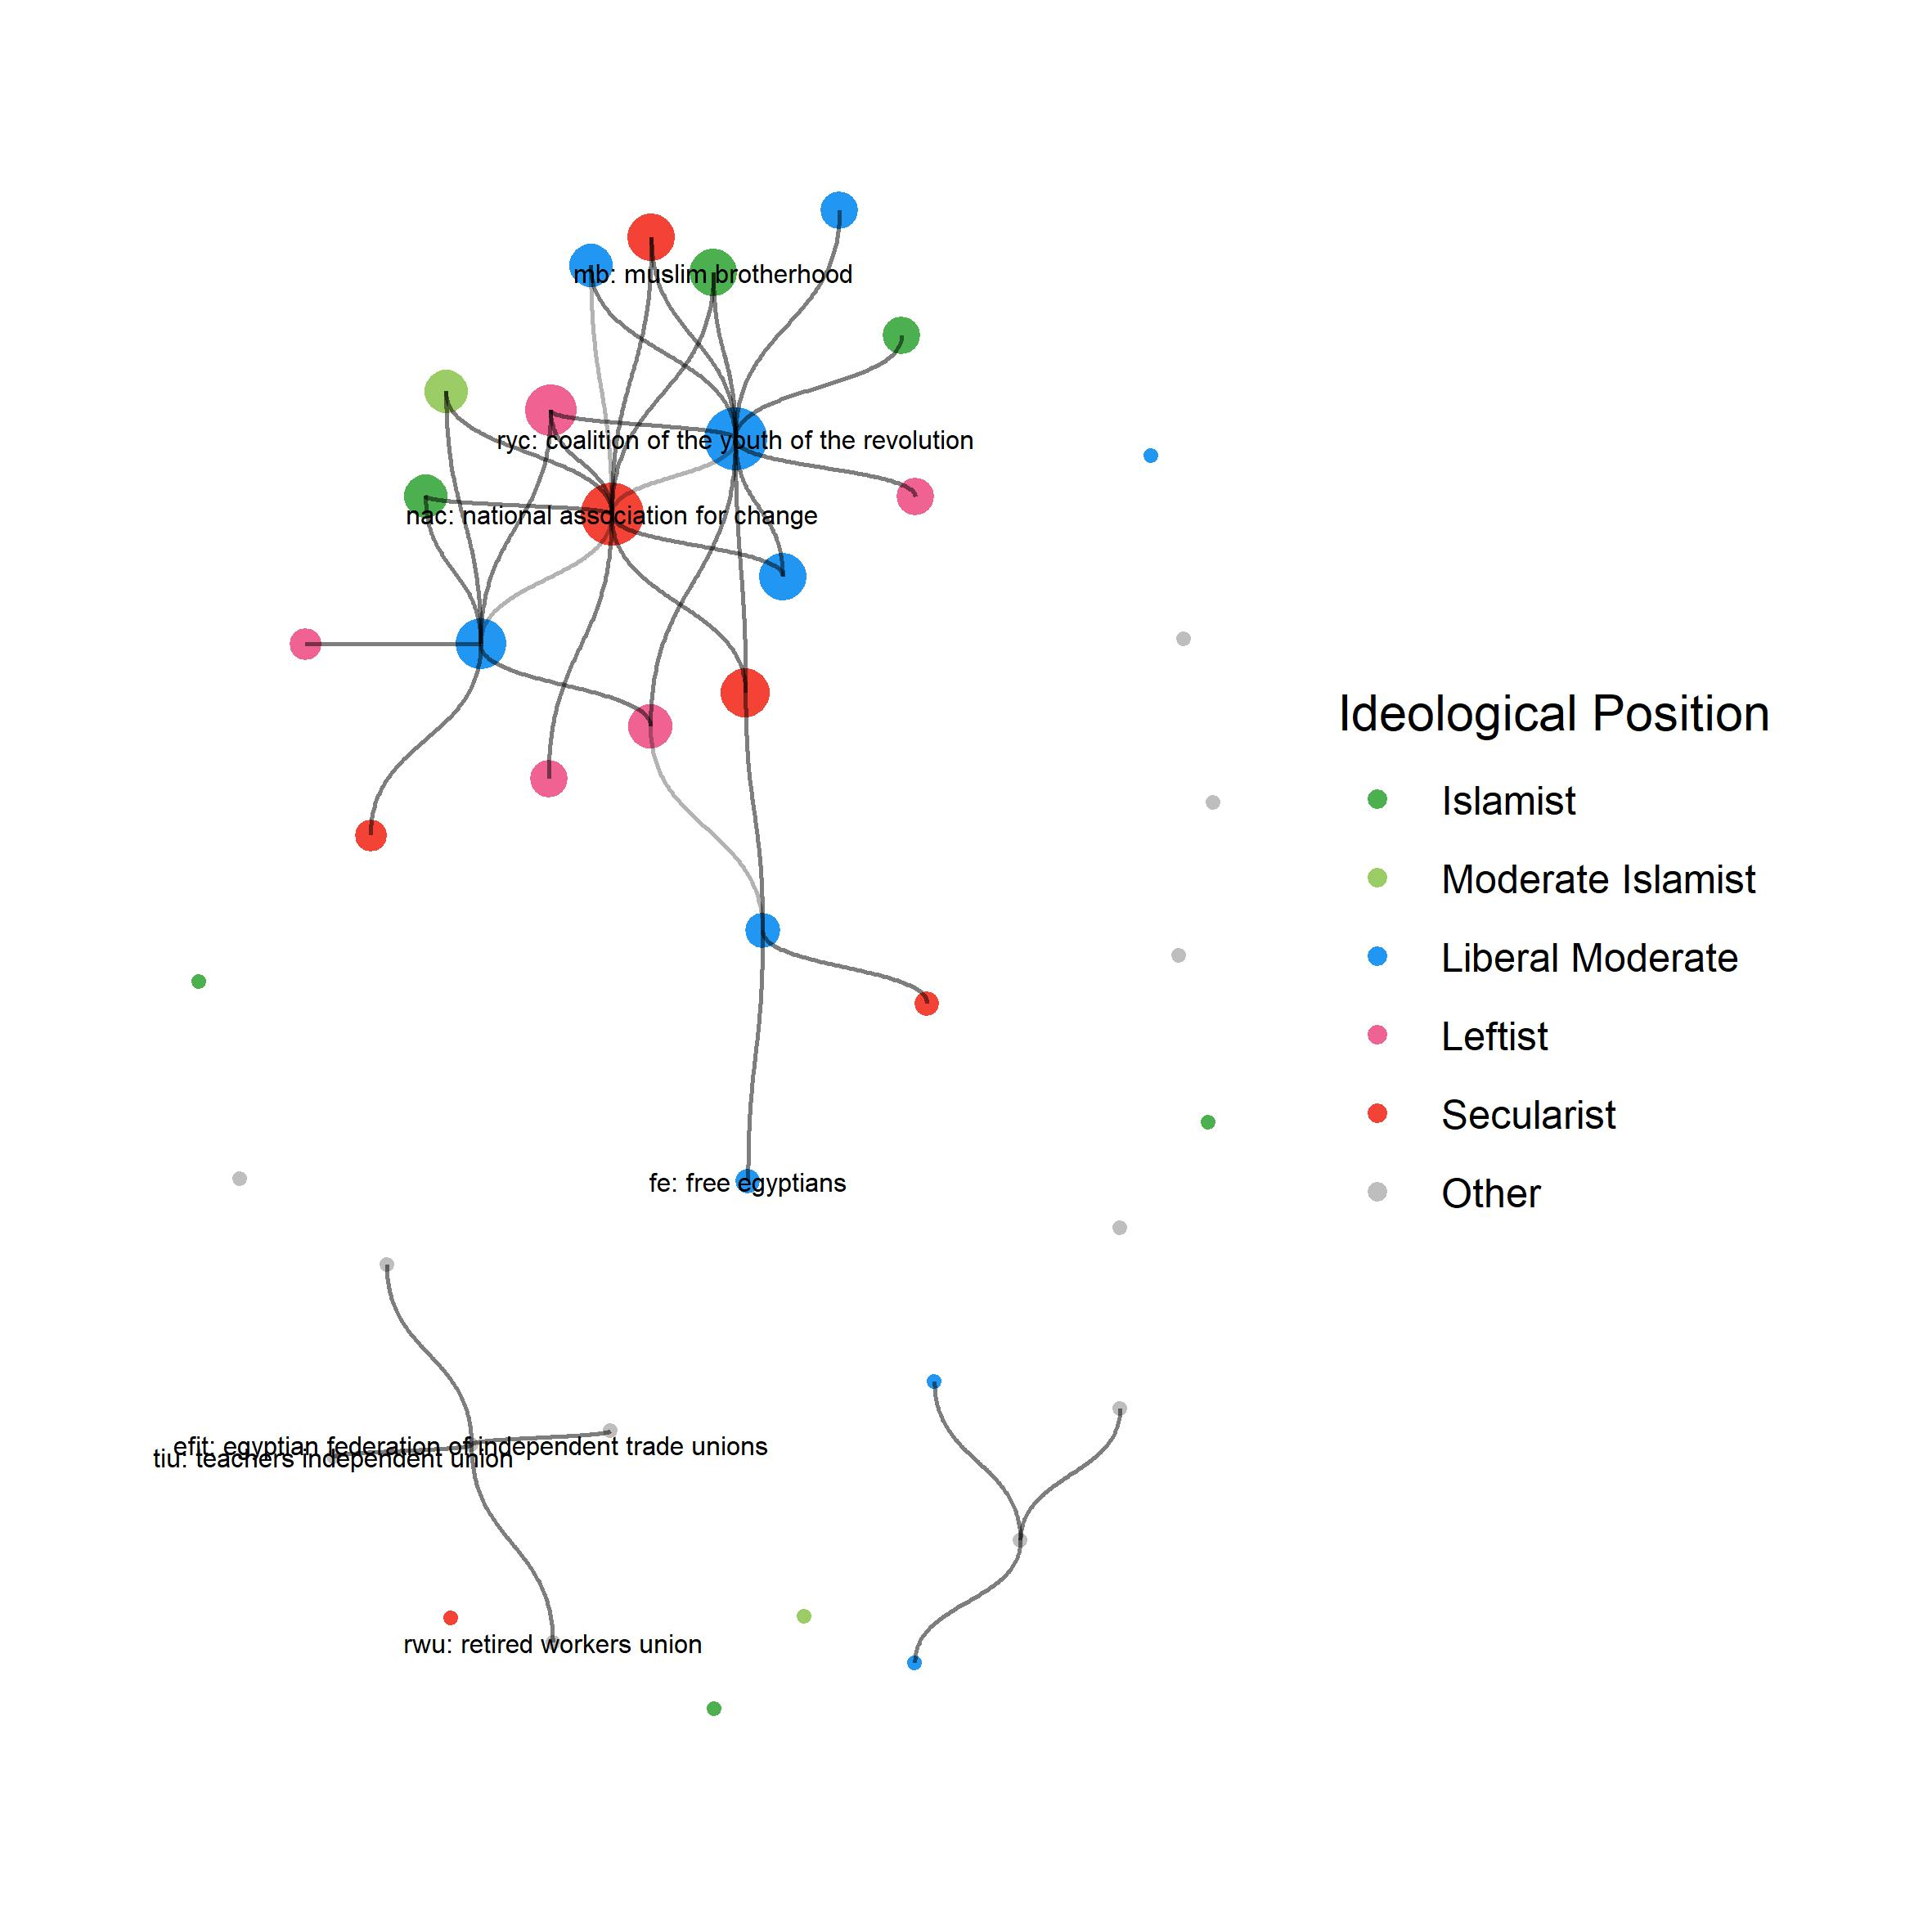
\includegraphics[width = 1.1\columnwidth]{img/egypt_2011.jpg}
    \caption{Egypt 2011$^g$ \\
        \footnotesize{$^g$Node sizes are proportional to degree centrality. Ideological positions were generated with text-matching on the organization-goals variable (see Appendix). Named organizations have a centrality score over $>0.6$ or an estimated membership size of more than 100,000}
}
    \label{Fig: Net1}
\end{figure}


\clearpage

\section{Descriptive statistics}

Political parties and rebel groups\footnote{We use the term rebel group to
characterize armed groups explicitly organized to challenge the state using
violence; this does not require involvement in conflicts with 25+ battle deaths
as with UCDP coding rules, but rather follows the logic of \citet{Lewis2020}.}
are the most common types of organizations in ARC. Figure \ref{fig:dotplot}
shows the number of organizations in maximalist dissent by year and country.
Stretches of little dissent are sometimes followed by bursts (Burkina Faso),
while the number of organizations in dissent escalates over time in other cases
(Sudan). Some countries exhibit consistently high numbers of organizations in
dissent (Ethiopia) while others are stable and low (Namibia). 

\begin{figure}[!htbp]
    \centering
    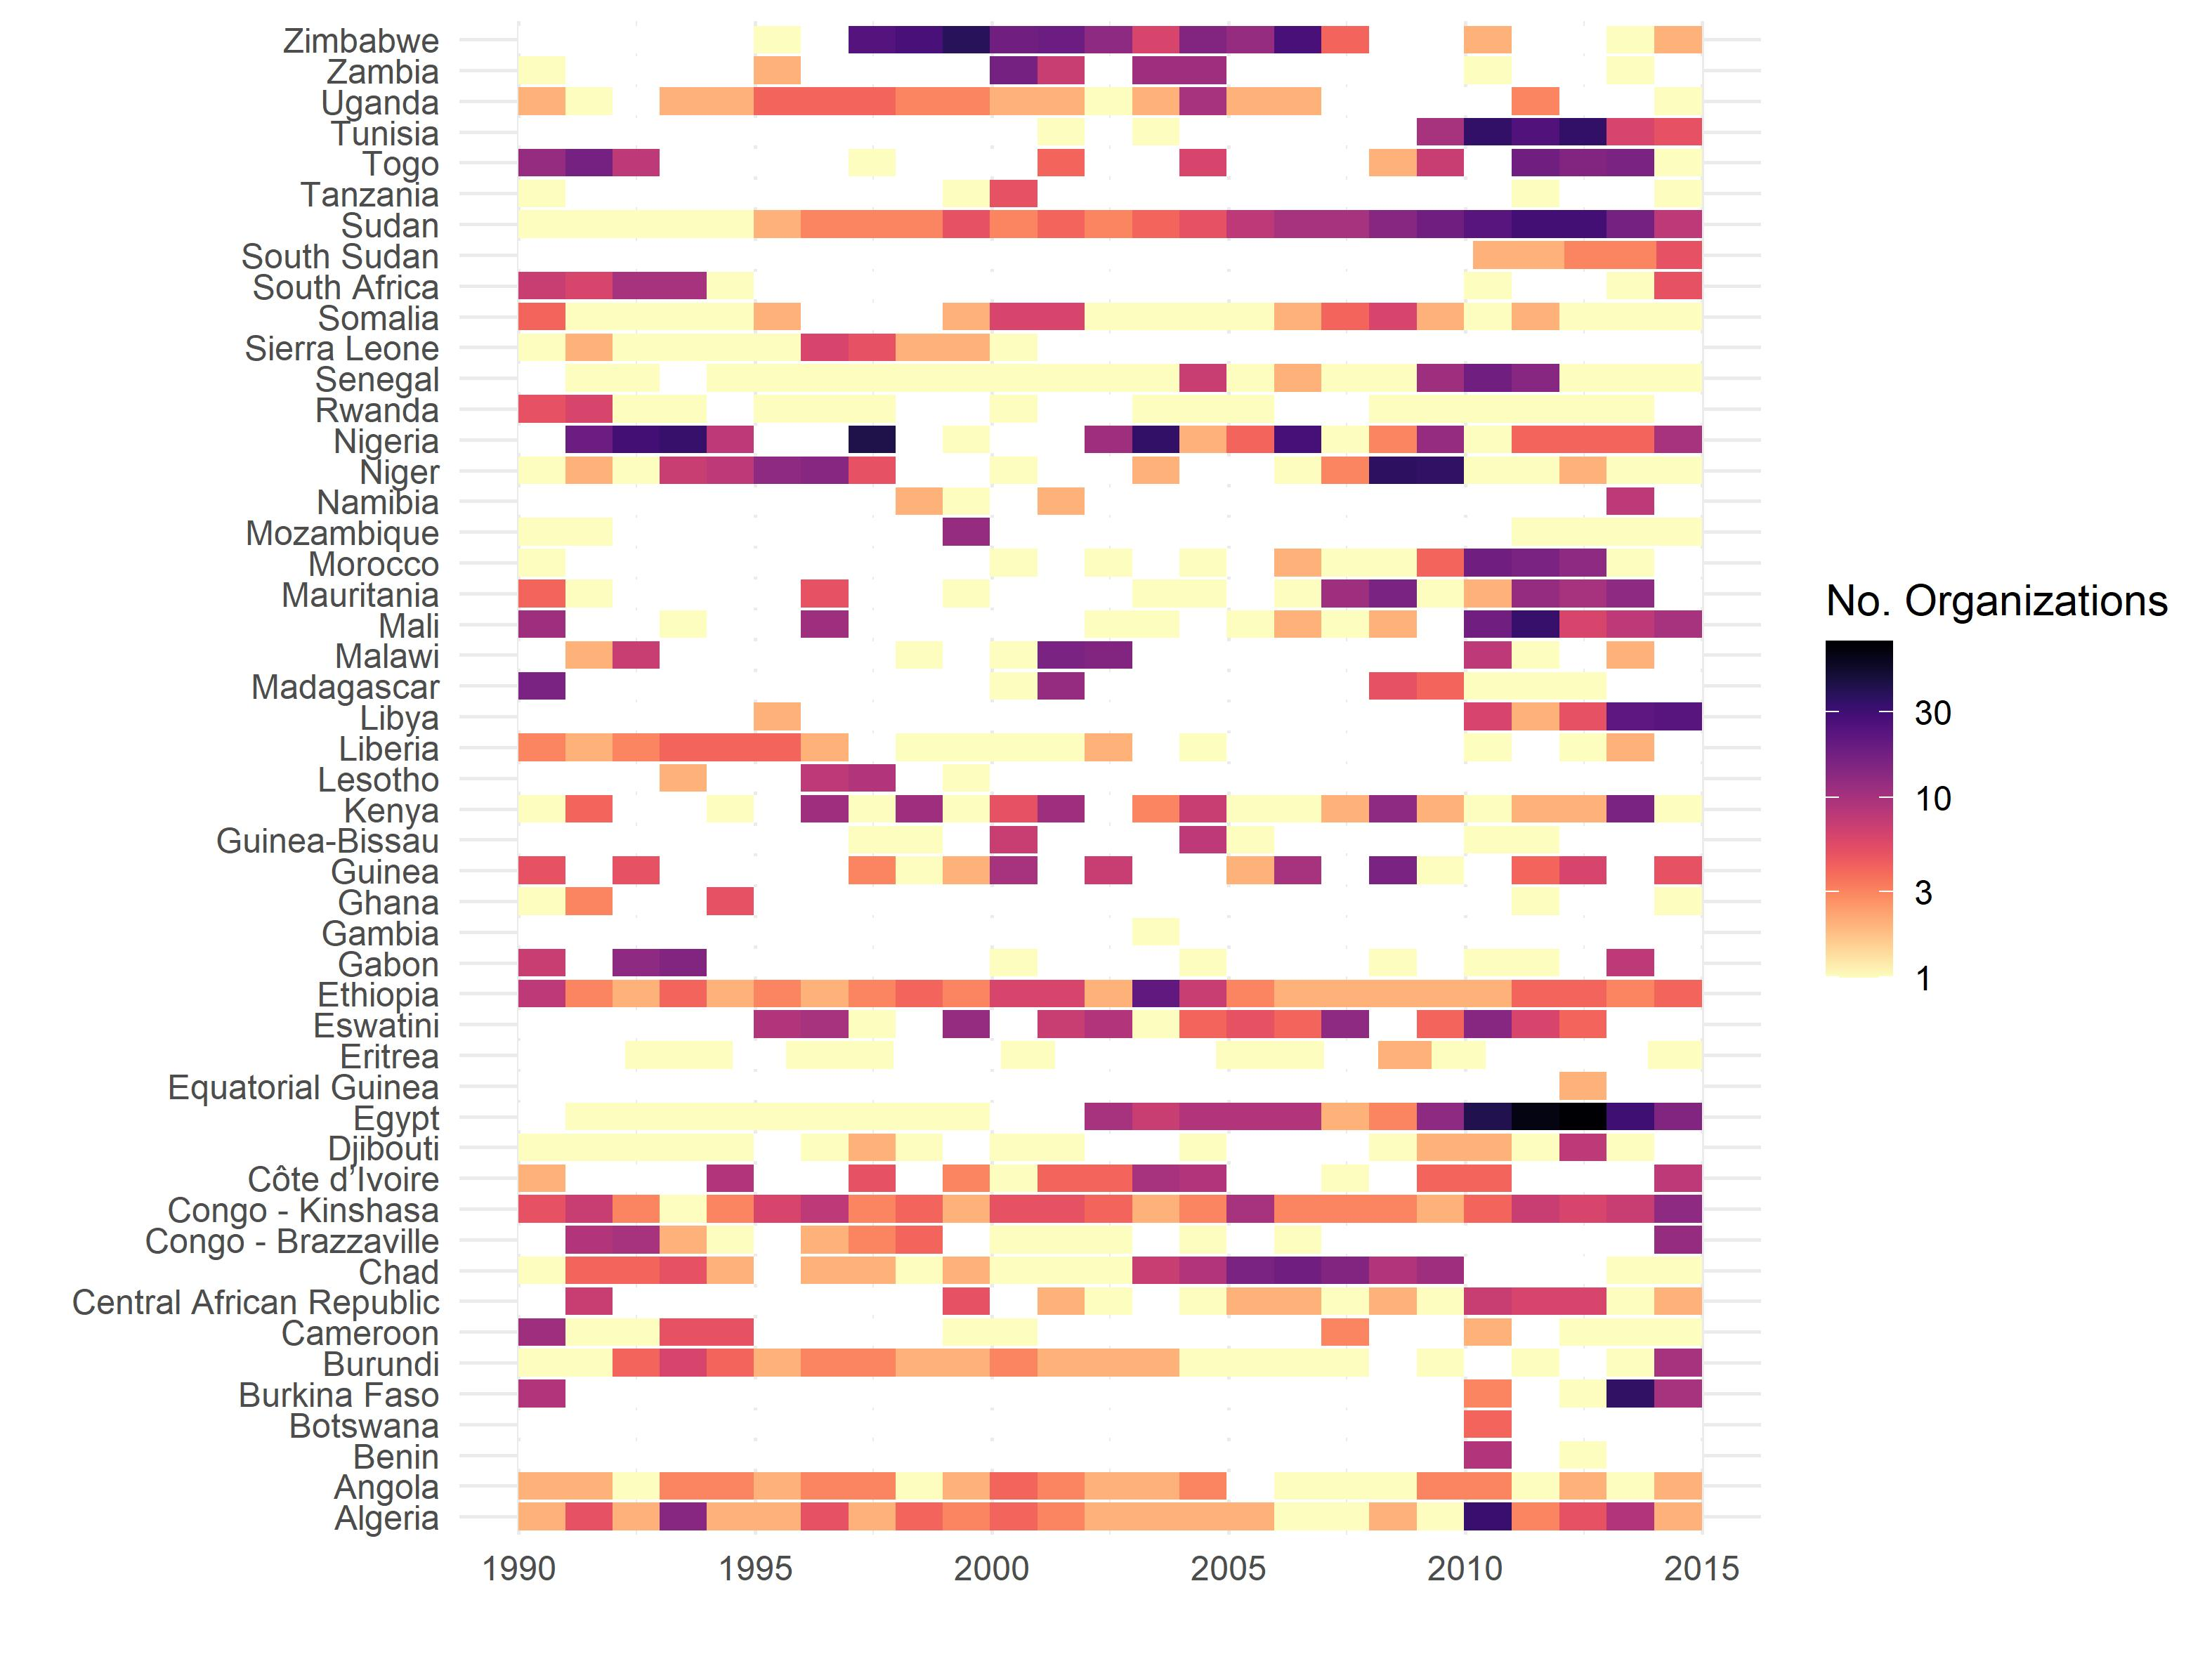
\includegraphics[width = 1\textwidth]{img/figure_2_revised.jpg}
    \caption{ARC organizations over time and space}
    \label{fig:dotplot}
\end{figure}{}


Table \ref{Tab: Types} shows how ARC variables vary across organization types. 

\begin{landscape}

\pagestyle{plain}

\begin{table}[!htbp] \centering 
  \caption{Features of Organization-Years in Resistance by Type} 
  \label{Tab: Types} 
\scalebox{.8}{
\begin{tabular}{cccccccccccc} 
\\[-1.8ex]\hline 
\hline \\[-1.8ex] 
Type & N & N Unique Orgs. & Splinter & Size Estimate & Age & Included in Regime & Legal & \# Ties & Female Leader & Decentralized & Alliances \\ 
\hline \\[-1.8ex] 
Pol. Party & 1143 & 532 & 0.27 & 3 & 6.51 & 0.08 & 0.7 & 1.2 & 0.02 & 0.05 & NA \\ 
Trade Union & 214 & 96 & 0.16 & 4 & 24.06 & 0.06 & 0.83 & 1.87 & 0.05 & 0.63 & NA \\ 
Religious & 101 & 42 & 0 & 3 & 32.85 & 0.02 & 0.95 & 1.38 & 0 & 0.63 & NA \\ 
Student/Youth & 69 & 27 & 0.09 & 3 & 17.62 & 0.03 & 0.55 & 1.52 & 0 & 0.25 & NA \\ 
Front & 262 & 157 & 0.01 & 3 & 2.01 & 0.03 & 0.33 & 6.67 & 0.06 & 0.87 & NA \\ 
Other CSO & 558 & 297 & 0.08 & 2 & 10.13 & 0.01 & 0.72 & 1.51 & 0.19 & 0.21 & NA \\ 
Rebel & 1004 & 273 & 0.4 & 3 & 7.63 & 0.02 & 0.03 & 1.32 & 0 & 0.26 & NA \\ 
Other & 44 & 26 & 0.2 & 3 & 9.65 & 0.02 & 0.5 & 1 & 0.13 & 0.25 & NA \\ 
Missingness (\%) &  &  & 0.12 & 0.17 & 0.08 & 0.03 & 0.03 & NA & 0.12 & 0.01 & 0.01 \\ 
\hline \\[-1.8ex] 
\multicolumn{12}{l}{\makecell[l]{All summary statistics are means except for the Size
Estimate which is a median. \textit{Included} measures whether the organization
was formally\\ or informally included in the governing coalition at $t-1$}} \\ 
\end{tabular} 
}
\end{table} 


\end{landscape}


Rebel groups and parties commonly split from other organizations. Rebel groups
dissent for longer (3.6 years on average) and more continuously (they have the
lowest variance around the mean participation year) than other organizations.
Participation by other types of organizations in ARC is ``bursty,'' perhaps
concentrated around elections or other focal points. Trade unions tend to be
large, old, and more connected to the state and other opposition organizations
than most other organizations. As one would expect, fronts are the most highly
connected, with ties to 5.67 other organizations on average. Only CSOs have
moderate levels of female leadership. Decentralization is most common in fronts,
religious groups, and trade unions.

\section{Correlates of organizational participation}

Different types of organizations should have distinct correlates of
participation in resistance given their varied constituencies and
goals.\footnote{Models were run in R 4.0.2} We explore associations between
socioeconomic factors and the number of organizations of different types active
in maximalist dissent using Negative Binomial models for over-dispersed count
data. Specifically, we examine inequality, economic modernization,
industrialization, economic growth, natural resource wealth, democratic
institutions, the number of other participating dissident organizations of
various types and a lagged dependent variable. Past research highlights these
possible explanations for participation in maximalist dissent
\citep{Acemoglu2005, Ansell2014, Ross2001, BuenoDeMesquita2010, Haggard2016,
maves2013, Aksoy2012}.  


Income inequality (and its square) is captured using Gini
coefficients.\footnote{Data come from the World Bank unless indicated
otherwise.} Economic development is measured with GDP per capita in constant
2000 USD, along with the GDP growth rate to proxy economic downturns.
Value-added manufacturing as a \% of GDP represents the strength of the
industrial sector \citep{Haggard2016, Butcher2016a} and oil revenues as a \% of
GDP proxy for natural resource dependency. We measure prior political
institutions with the V-DEM Polyarchy score \citep{Coppedge2019}, as well as its
square \citep{Hegre2006}. Repression is measured with the Physical Violence
Index, also from VDEM. These variables are lagged one year. The number of
organizations of other types engaged in maximalist dissent in year $t$ is
included to explore patterns of co-participation across organization-types. 

Table \ref{Tab: Structure} presents our findings. Visualizations can be found in
the Appendix. The results for economic development are striking. More rebel
groups mobilize in poorer countries, while more trade unions, student
organizations, and other CSOs dissent in more developed countries. Broad,
labor-based civil society coalitions may be an important link in the chain from
modernization to democracy \citep{Chenoweth2011, Celestino2013, Bayer2016,
Dahlum2019, Boix2003a}. Movements underpinned by thinner, technology-driven
networks may be more brittle \citep{Weidmann2018}. Oil dependency is associated
with fewer trade unions, student groups, ``other'' organizations, and religious
organizations engaging in maximalist dissent, but more active rebel groups.
These models are a first, descriptive look at patterns of participation that say
little about the deeper mechanisms, however. For example, structural factors may
alter the underlying organizational ecology, drive participation in maximalist
dissent directly, or activate other processes, such as splintering. 

Structural variables appear to be poor predictors of the number of fronts in
dissent. Coalition formation may occur after shorter term shocks related to food
prices \citep{Abbs2020} or severe repression events \citep{Chang2008}. This is
worth investigating in future work. Models addressing censorship and
international media coverage (in the appendix) do not indicate strong media
biases across most organization types.

\pagebreak

\begin{table}[!htbp]
\begin{center}
\scalebox{0.65}{
\begin{tabular}{l c c c c c c c c}
\hline
 & Political Parties & Trade Unions & Rel. Orgs & Student/Youth & Fronts & Rebel Groups & Other CSOs & Others \\
\hline
Oil (\% GDP)                 & $-0.01$        & $-0.09^{**}$ & $-0.27^{**}$  & $-0.08^{*}$  & $-0.01$       & $0.03^{***}$  & $-0.02$       & $-0.61^{**}$ \\
                             & $(0.01)$       & $(0.03)$     & $(0.09)$      & $(0.03)$     & $(0.01)$      & $(0.01)$      & $(0.01)$      & $(0.23)$     \\
Manufacturing (\% GDP)       & $0.02$         & $0.00$       & $0.09$        & $0.13^{***}$ & $-0.01$       & $0.02^{*}$    & $0.01$        & $0.07$       \\
                             & $(0.01)$       & $(0.02)$     & $(0.05)$      & $(0.03)$     & $(0.02)$      & $(0.01)$      & $(0.02)$      & $(0.07)$     \\
Polyarchy                    & $7.19^{**}$    & $-2.23$      & $17.24$       & $1.76$       & $2.79$        & $-1.65$       & $6.12$        & $12.46$      \\
                             & $(2.52)$       & $(5.19)$     & $(9.88)$      & $(6.40)$     & $(2.86)$      & $(1.68)$      & $(3.84)$      & $(11.00)$    \\
Polyarchy $^2$               & $-10.26^{***}$ & $0.42$       & $-29.11^{*}$  & $0.31$       & $-3.96$       & $1.16$        & $-5.76$       & $-16.34$     \\
                             & $(2.95)$       & $(5.79)$     & $(12.07)$     & $(7.68)$     & $(3.30)$      & $(2.05)$      & $(4.20)$      & $(12.70)$    \\
Income Inequality $^2$       & $0.00$         & $-0.00$      & $-0.00$       & $-0.00$      & $-0.00$       & $-0.00$       & $-0.00$       & $0.00$       \\
                             & $(0.00)$       & $(0.00)$     & $(0.00)$      & $(0.00)$     & $(0.00)$      & $(0.00)$      & $(0.00)$      & $(0.00)$     \\
Income Inequality            & $-0.03$        & $0.10$       & $0.11$        & $0.20$       & $0.09$        & $-0.04$       & $0.24$        & $-0.43$      \\
                             & $(0.09)$       & $(0.18)$     & $(0.28)$      & $(0.22)$     & $(0.10)$      & $(0.06)$      & $(0.13)$      & $(0.27)$     \\
Log GDP per Capita           & $0.03$         & $0.79^{**}$  & $-0.33$       & $0.85^{**}$  & $0.12$        & $-0.51^{***}$ & $0.58^{**}$   & $0.94^{*}$   \\
                             & $(0.13)$       & $(0.26)$     & $(0.41)$      & $(0.33)$     & $(0.13)$      & $(0.09)$      & $(0.18)$      & $(0.47)$     \\
GDP Growth                   & $0.81$         & $-4.24^{*}$  & $-1.07$       & $-0.42$      & $-0.29$       & $0.09$        & $-1.28$       & $4.66$       \\
                             & $(0.87)$       & $(1.87)$     & $(3.21)$      & $(1.97)$     & $(0.94)$      & $(0.53)$      & $(1.39)$      & $(4.06)$     \\
Physical Integrity Rights    & $0.02$         & $0.33$       & $0.30$        & $-4.96^{**}$ & $-0.96$       & $-0.40$       & $-1.40^{*}$   & $-3.90^{*}$  \\
                             & $(0.46)$       & $(0.92)$     & $(1.70)$      & $(1.55)$     & $(0.53)$      & $(0.33)$      & $(0.71)$      & $(1.76)$     \\
Year                         & $0.01$         & $0.04$       & $0.14^{**}$   & $0.03$       & $-0.01$       & $0.00$        & $0.08^{***}$  & $0.07$       \\
                             & $(0.01)$       & $(0.02)$     & $(0.04)$      & $(0.03)$     & $(0.01)$      & $(0.01)$      & $(0.02)$      & $(0.04)$     \\
Population (Log)             & $0.08$         & $-0.28^{*}$  & $0.47$        & $0.13$       & $0.04$        & $0.26^{***}$  & $0.39^{***}$  & $0.78^{*}$   \\
                             & $(0.07)$       & $(0.14)$     & $(0.30)$      & $(0.20)$     & $(0.08)$      & $(0.05)$      & $(0.10)$      & $(0.34)$     \\
No. Political Parties        &                & $0.11^{*}$   & $0.31^{***}$  & $-0.01$      & $0.19^{***}$  & $-0.01$       & $0.10^{**}$   & $0.02$       \\
                             &                & $(0.05)$     & $(0.08)$      & $(0.04)$     & $(0.02)$      & $(0.02)$      & $(0.04)$      & $(0.06)$     \\
No. Trade Unions             & $0.06$         &              & $-0.01$       & $0.28^{**}$  & $0.29^{***}$  & $0.00$        & $0.39^{***}$  & $0.25$       \\
                             & $(0.09)$       &              & $(0.23)$      & $(0.10)$     & $(0.05)$      & $(0.08)$      & $(0.10)$      & $(0.20)$     \\
No. Rel. Orgs                & $0.15$         & $0.23^{*}$   &               & $0.24^{*}$   & $0.15^{*}$    & $-0.18$       & $0.41^{***}$  & $0.21$       \\
                             & $(0.09)$       & $(0.12)$     &               & $(0.10)$     & $(0.07)$      & $(0.14)$      & $(0.09)$      & $(0.14)$     \\
No. Student/Youth Orgs       & $-0.07$        & $0.44$       & $0.02$        &              & $-0.24$       & $-0.28$       & $0.61^{**}$   & $-0.20$      \\
                             & $(0.23)$       & $(0.28)$     & $(0.55)$      &              & $(0.17)$      & $(0.17)$      & $(0.23)$      & $(0.37)$     \\
No. Fronts                   & $1.71^{***}$   & $0.88^{***}$ & $0.38$        & $0.16$       &               & $0.11$        & $0.93^{***}$  & $0.18$       \\
                             & $(0.12)$       & $(0.18)$     & $(0.36)$      & $(0.18)$     &               & $(0.09)$      & $(0.17)$      & $(0.41)$     \\
No. Rebel Groups             & $-0.17^{***}$  & $-0.19$      & $-0.18$       & $0.25^{***}$ & $0.25^{***}$  &               & $-0.27^{***}$ & $-0.01$      \\
                             & $(0.04)$       & $(0.11)$     & $(0.23)$      & $(0.05)$     & $(0.03)$      &               & $(0.07)$      & $(0.24)$     \\
No. CSOs                     & $0.01$         & $0.16^{***}$ & $0.51^{***}$  & $0.10^{**}$  & $0.09^{***}$  & $0.00$        &               & $0.15^{**}$  \\
                             & $(0.03)$       & $(0.04)$     & $(0.08)$      & $(0.03)$     & $(0.02)$      & $(0.03)$      &               & $(0.06)$     \\
No. Others                   & $-0.40^{*}$    & $-0.52^{*}$  & $-2.53^{***}$ & $0.01$       & $-0.55^{***}$ & $0.12$        & $-0.53^{*}$   &              \\
                             & $(0.20)$       & $(0.25)$     & $(0.52)$      & $(0.20)$     & $(0.13)$      & $(0.15)$      & $(0.21)$      &              \\
No. Political Parties (t-1)  & $0.11^{***}$   &              &               &              &               &               &               &              \\
                             & $(0.02)$       &              &               &              &               &               &               &              \\
No. Trade Unions (t-1)       &                & $0.33^{***}$ &               &              &               &               &               &              \\
                             &                & $(0.10)$     &               &              &               &               &               &              \\
No. Rel. Orgs (t-1)          &                &              & $0.47^{**}$   &              &               &               &               &              \\
                             &                &              & $(0.17)$      &              &               &               &               &              \\
No. Student/Youth Orgs (t-1) &                &              &               & $0.38^{*}$   &               &               &               &              \\
                             &                &              &               & $(0.18)$     &               &               &               &              \\
No. Fronts (t-1)             &                &              &               &              & $-0.08$       &               &               &              \\
                             &                &              &               &              & $(0.09)$      &               &               &              \\
No. Rebel Groups (t-1)       &                &              &               &              &               & $0.29^{***}$  &               &              \\
                             &                &              &               &              &               & $(0.02)$      &               &              \\
No. CSOs (t-1)               &                &              &               &              &               &               & $0.07^{*}$    &              \\
                             &                &              &               &              &               &               & $(0.03)$      &              \\
No. Others (t-1)             &                &              &               &              &               &               &               & $0.37^{*}$   \\
                             &                &              &               &              &               &               &               & $(0.19)$     \\
\hline
AIC                          & $1918.39$      & $606.68$     & $334.35$      & $270.20$     & $798.84$      & $1743.83$     & $1018.85$     & $177.61$     \\
BIC                          & $2020.66$      & $708.95$     & $436.62$      & $372.47$     & $901.11$      & $1846.10$     & $1121.12$     & $279.88$     \\
Log Likelihood               & $-938.19$      & $-282.34$    & $-146.17$     & $-114.10$    & $-378.42$     & $-850.91$     & $-488.42$     & $-67.81$     \\
Deviance                     & $592.27$       & $202.48$     & $85.70$       & $128.22$     & $359.43$      & $699.10$      & $332.07$      & $84.89$      \\
Num. obs.                    & $963$          & $963$        & $963$         & $963$        & $963$         & $963$         & $963$         & $963$        \\
\hline
\multicolumn{9}{l}{\scriptsize{$^{***}p<0.001$; $^{**}p<0.01$; $^{*}p<0.05$}}
\end{tabular}
}
\caption{Correlates of Organizational Participation}
\label{Tab: Structure}
\end{center}
\end{table}

\pagebreak

Table \ref{Tab: Structure} also reveals patterns of organizational
cross-participation. Parties mobilize with fronts, but alongside fewer rebel
groups. Trade unions and CSOs dissent alongside one another and with more
parties, religious organizations, and fronts. Religious organizations have
narrower co-participation profiles, mobilizing alongside other CSOs. Student
groups dissent alongside rebel groups, in addition to trade unions, religious
organizations, and other CSOs. Rebel groups tend to act without high numbers of
other types of organizations. Finally, fronts assemble many group types
including parties, rebels, trade unions, religious organizations, and other
CSOs.

These findings highlight the usefulness of ARC for (re)examining mechanisms
highlighted in theories of social change, as well as the ability to uncover
novel, previously un(der)theorized relationships.

\section{Conclusion}

The ARC dataset advances our understanding of anti-government mobilization and
has many potential applications. ARC provides details about organizations that
engaged in violent and nonviolent dissent at various periods of their existence
and could be used to identify correlates of tactical shifts. ARC should be
useful to scholars of repression and dissent; connections to events datasets
facilitate exploration of how organizational networks interact with repression
to produce backlash and demobilization. ARC can also be collapsed into
country-year format and merged with data on campaign outcomes (e.g.
\citet{Chenoweth2019a}, \citet{Kreutz2010}), regime change, and democratization
\citep{Goemans2009, Djuve2020, Coppedge2019}. Information on
inter-organizational ties can be used to generate network maps that span
conventional violent-nonviolent dichotomies and even link campaigns
cross-nationally. We look forward to seeing how others engage ARC to expand our
knowledge of the causes, dynamics, and consequences of maximalist dissent.

\pagebreak


\textbf{Acknowledgements:} We thank Alice Dalsj\o, Nina Bj\o rge, Xiran Chen,
Stephanie Clinch, Tyler DeMers, Kelly Gordell, and Luna Ruiz for valuable
research assistance. For valuable comments and feedback we thank three anonymous
reviewers, Nils Metternich, Scott Gates, Janet Lewis, Kristian Skrede Gleditsch,
participants at the 2017 Peace Research Society Workshop on Conflict Networks,
the NTNU VIP seminars, participants in the SECVIC workshops, the 2019 workshop
on Actors and Conflict Processes at NTNU and the 2019 workshop on `Introducing
ARC' at the Conflict Research Society annual meeting at the University of
Sussex.\\

\textbf{Funding:} We gratefully acknowledge funding from the Norwegian Research
Council, the United States Institute of Peace and support grants from the
Department and Faculty at NTNU. Braithwaite received funding from USIP prior to
Pinckney accepting a position at USIP.  

\section{Author Bios}

Charles Butcher, b. 1982, PhD in Government and International Relations
(Sydney); Associate Professor, NTNU (2016-); Senior Researcher, PRIO (2018-). \\

Jessica Maves Braithwaite, b. 1986, PhD in Political Science (Pennsylvania State
University, 2013); Associate Professor, University of Arizona (2013– ); research
interests: civil war, nonviolent resistance, state repression, peacebuilding.\\

Jonathan Pinckney, b. 1986, PhD in International Relations (Denver, 2018);
Post-Doctoral Research Fellow, NTNU (2018 – 2019); Senior Researcher, United
States Institute of Peace (2019 - ); Most recent book: From Dissent to
Democracy: The Promise and Peril of Civil Resistance Transitions (Oxford,
2020).\\

Eirin Haugseth, b. 1993, MSc in Political Science (NTNU, 2020); Doctoral
Researcher, PRIO (2021–); current main interests: forced migration and social
unrest.\\

Ingrid Vik Bakken, b. 1991, MSc in Political Science (NTNU, 2017); PhD candidate
(NTNU, 2018 -- ).\\

Marius Swane Wishman, b. 1990, MA in Political Science (University in Tromsø);
PhD in Political Science, NTNU (2017- ).\\


\clearpage

\bibliographystyle{apsr}
\bibliography{jpr_bibliography_final.bib}

\clearpage

\section{Appendix}

\subsection{Models with Indicators of Government Censorship and International Media coverage}

The models below include two measures capturing aspects of the media environment
at the country year level. The first is ``Government Censorship Effort'' from
the VDEM dataset \citep{Coppedge2019}. Low values indicate that the media is
highly censored while higher values indicate higher levels of media freedom. The
second is a count of the number of Agence France Press and Associated Press
newswire hits that are obtained with the country name in the headline or lead
paragraph over a country-year. Chad is not included in these models because we
were unable to create a search string that reliably separated the country `Chad'
from the personal name Chad. The results for other variables in the model are
very similar to those in the main text, and we have excluded them from the table
to focus on the media-related variables. 

\begin{table}[!htpb]
\begin{center}
\scalebox{0.65}{
\begin{tabular}{l c c c c c c c c}
\hline
 & Political Parties & Trade Unions & Rel. Orgs & Student/Youth & Fronts & Rebel Groups & Other CSOs & Others \\
\hline                               &                &              &               &              &               &               &              & $(0.19)$    \\
Count of FACTIVA newswire hits & $0.00$         & $-0.00^{**}$ & $0.00$        & $-0.00$      & $0.00$        & $0.00$        & $-0.00$      & $0.00$      \\
                               & $(0.00)$       & $(0.00)$     & $(0.00)$      & $(0.00)$     & $(0.00)$      & $(0.00)$      & $(0.00)$     & $(0.00)$    \\
Media Freedom from Censorship  & $-0.09$        & $0.55$       & $-0.50$       & $-0.01$      & $-0.02$       & $0.44^{***}$  & $0.08$       & $-0.94$     \\
                               & $(0.14)$       & $(0.29)$     & $(0.44)$      & $(0.43)$     & $(0.16)$      & $(0.09)$      & $(0.21)$     & $(0.58)$    \\
\hline
AIC                            & $1790.60$      & $576.89$     & $333.12$      & $261.24$     & $709.52$      & $1413.08$     & $973.53$     & $166.32$    \\
BIC                            & $1901.20$      & $687.50$     & $443.73$      & $371.85$     & $820.13$      & $1523.69$     & $1084.13$    & $276.93$    \\
Log Likelihood                 & $-872.30$      & $-265.45$    & $-143.56$     & $-107.62$    & $-331.76$     & $-683.54$     & $-463.76$    & $-60.16$    \\
Deviance                       & $563.27$       & $190.93$     & $86.41$       & $123.25$     & $300.15$      & $593.42$      & $316.11$     & $71.55$     \\
Num. obs.                      & $906$          & $906$        & $906$         & $906$        & $906$         & $906$         & $906$        & $906$       \\
\hline
\multicolumn{9}{l}{\scriptsize{$^{***}p<0.001$; $^{**}p<0.01$; $^{*}p<0.05$}}
\end{tabular}
}
\caption{Correlates of Organizational Participation, Media Variables}
\label{Tab: Media}
\end{center}
\end{table}

\pagebreak

\subsection{Coding the Religious Diversity Measure in the Main text}

On pages 12 and 13 we show indicators of religious diversity over the years
2003-2015 in Egypt. These variables were generated from the ARC data with
text-matching in R (version 4.0.2) on the organization goals variable according
to the rules in the table below. The organization goals variable matches the
text-matching pattern if any one of the listed strings matches with the words in
the organization goals variable. For example, if any of the text in the
organization goals variable matched the strings \textit{secula} OR
\textit{antiislam} then this would return a positive match for the
\textit{Secularist} variable. White space and punctuation was removed from the
words before the text-matching was used.  

\begin{table}[!htbp] \centering 
  \caption{Organization Size Estimate} 
  \label{Tab: Table 1} 
\begin{tabular}{p{6cm} p{10cm}} 
\\[-1.8ex]\hline 
\hline \\[-1.8ex] 
Category & \multicolumn{1}{c}{Coding Rule} \\
\hline \\[-1.8ex] 
\emph{Islamist}     &   islam OR sharia OR jihad OR emirat OR salaf OR caliphat OR sunni OR muslim \\ 
\hline \\[-1.8ex] 
\emph{Moderate Islamist}     &   Islamist = TRUE and Liberal Moderate = TRUE  \\ 
\hline \\[-1.8ex] 
\emph{Moderate Liberal}     &   liberal OR moderat OR centr OR center OR democra OR civilandlegalrights OR multiparty OR egalitarian OR electionintegrity OR civilsociety OR equality OR humanrights OR freedom OR plural OR freeelections OR fairelections OR libert OR suffrage OR freepress OR progressive OR humanist OR inclus AND Islamist = FALSE AND Moderate Islamist = FALSE AND Secular = FALSE AND Leftist=FALSE AND Christian = FALSE \\ 
\hline \\[-1.8ex] 
\emph{Leftist}     &   left OR anticapitalist OR socialis OR marx OR lenin OR trotsky OR communis OR class OR redistribution OR anticapital OR nationalization OR nationalizedeconomy  \\ 
\hline \\[-1.8ex] 

\emph{Secularist}     &  secula OR antiislam AND Leftist = FALSE \\ 
\hline \\[-1.8ex] 

\emph{Christian}     &  christ OR evangel OR catholic OR gospel OR prosel OR biblic OR coptic  \\ 
\hline \\[-1.8ex] 

\emph{Other}     &  Does not match any of the above patterns  \\ 
\hline \\[-1.8ex] 


\hline \\[-1.8ex] 
\end{tabular} 
\end{table} 

\pagebreak

\subsection{Visualisations of the main results}

Below are two figures that visualise the main results from Table 4 in the main
text. Figure \ref{Fig: Main Results} plots the predicted number of organizations
of a given type for different values of the structural variables in the model.
These estimates were generated using the \texttt{ggeffects} package in
\texttt{R}. Figure \ref{Fig: Clusters} visualises organization types that tend
to participate together with a network graph, based on the results in Table 4
regarding how the participation of organization types is associated with the
participation on other organization type. Organization-types have ties between
them where we found a positive and statistically significant average marginal
effect between the participation of organization type $i$ and organization type
$j$. The width of the ties is proportional to the size of the average marginal
effects. Figure \ref{Fig: Clusters} shows that rebel groups and ``other''
organizations tend to act alone, while fronts are most strongly associated with
political party, trade union and ``Other CSO'' participation. Trade Unions tend
to participate with CSOs, which in turn have relatively strong associations with
the participation of religious groups and student/youth organizations.    

\begin{figure}[!htbp]
    \centering
    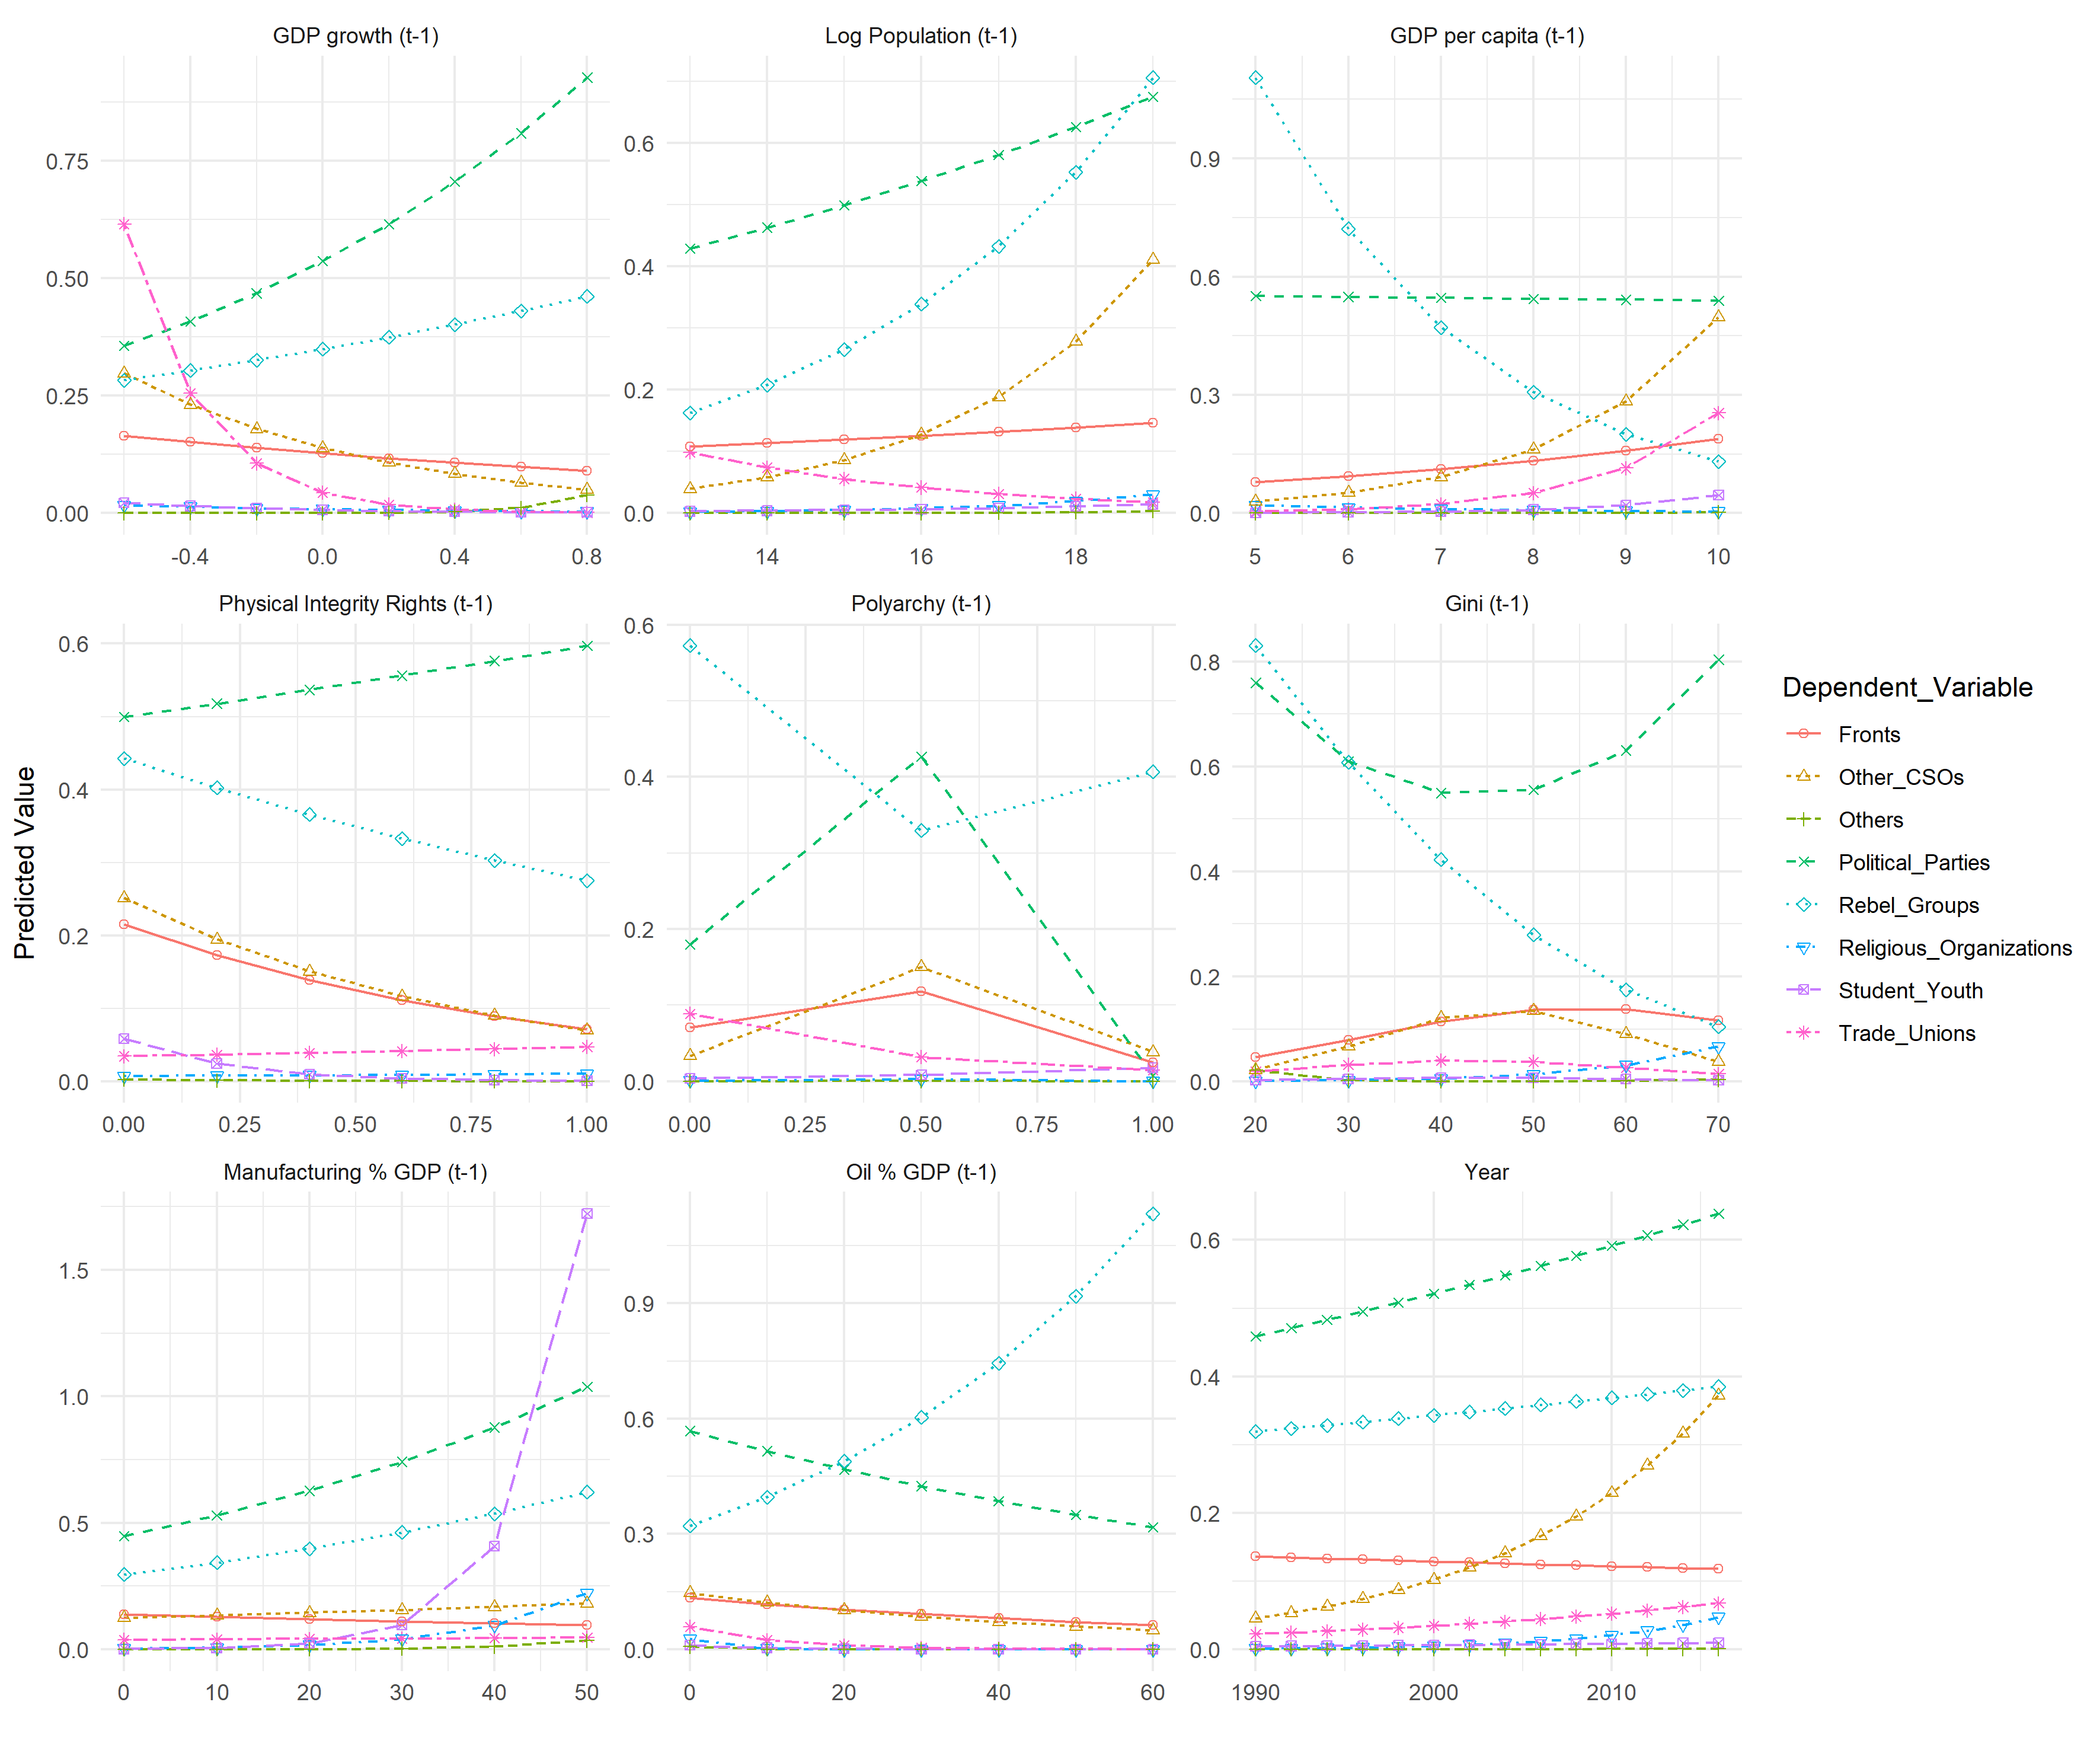
\includegraphics[width = 1\textwidth]{img/arc_margins_structural.png}
    \caption{Visualizations: Main Results in the Text, Structural Variables}
    \label{Fig: Main Results}
\end{figure}{}

\begin{figure}[!htpb]
    \centering
    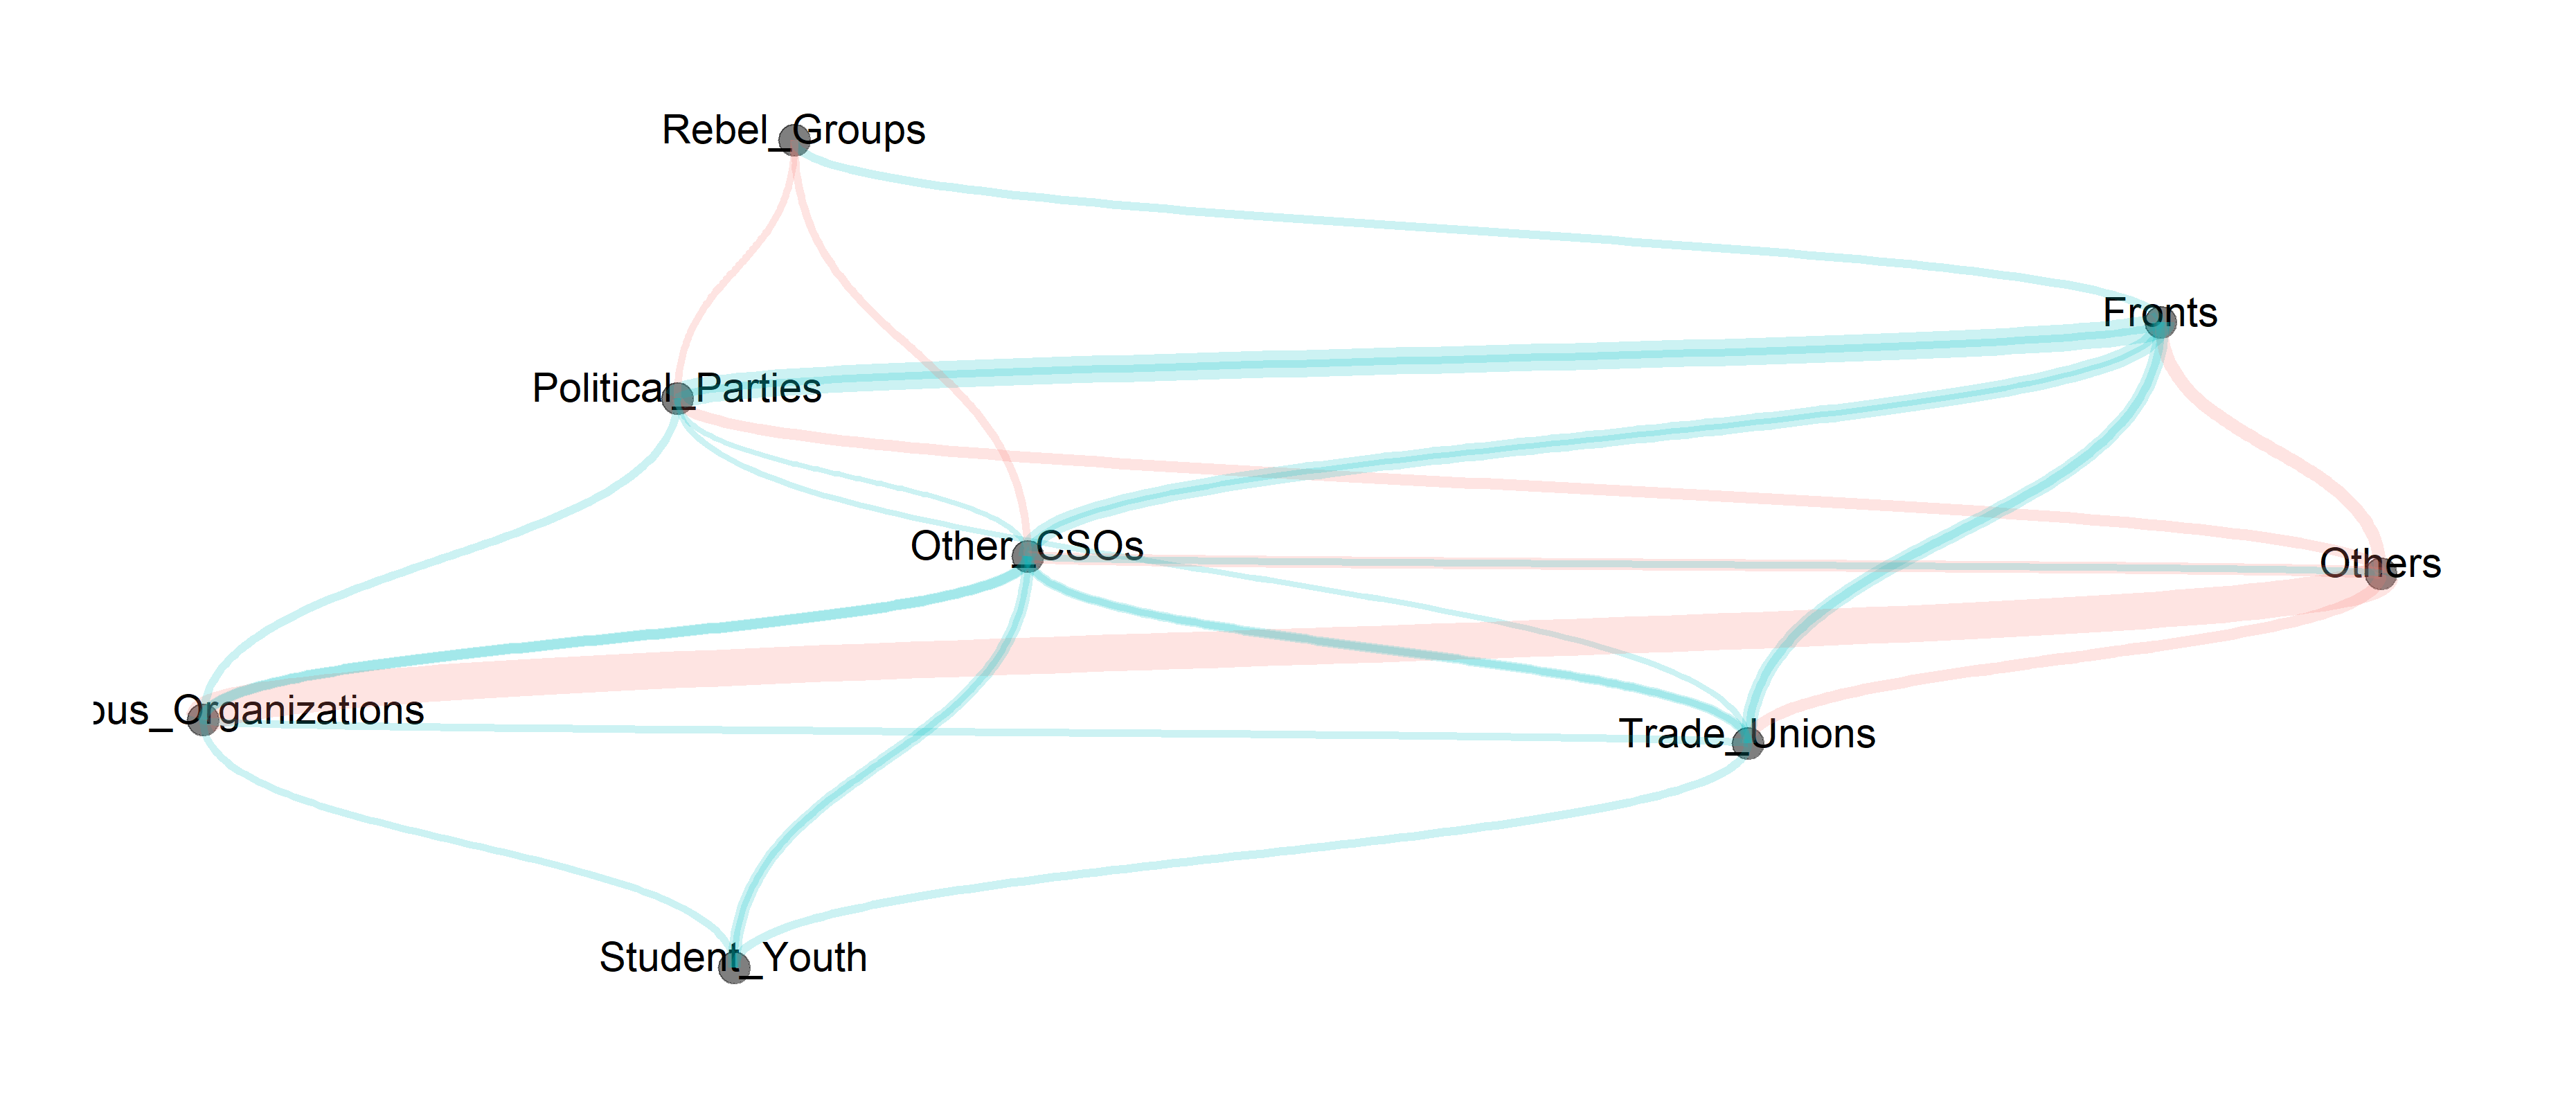
\includegraphics[width = 1\textwidth]{img/arc_network_clusters.png}
    \caption{Visualizations: Clustering of Organization Types in Country-Years}
    \label{Fig: Clusters}
\end{figure}{}

